\ofsubsection{Combat}
%
\ofquote{"Enough expository banter. It's time we fight like men. And ladies. And ladies who dress like men."\\}{Gilgamesh}\\
%
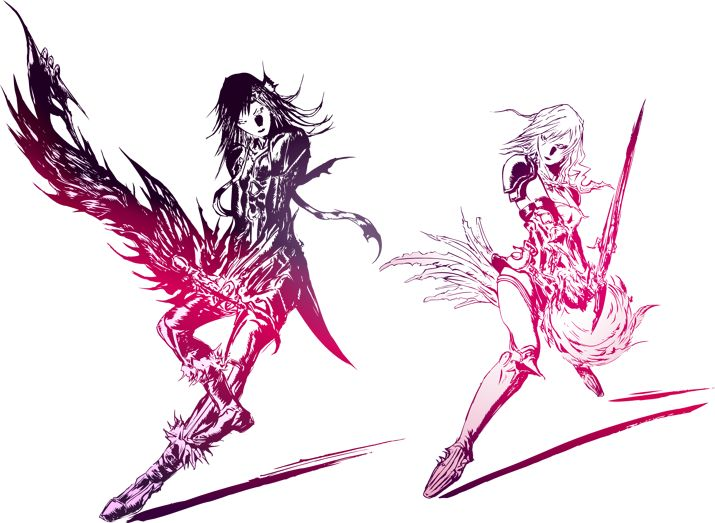
\includegraphics[width=\columnwidth]{./art/images/ff13-2.jpg}
%
\vfill
%
\ofboxwithtitle{Combat}{
Combat encounters play out in a series of rounds (shortened~\acc{r}) and during a round every combatant takes one turn.
In every round, the players take their turns first, they can freely decide in which order.
Then all enemy combatants take their turns until the round is concluded.
Rinse and repeat until one party is defeated.
When a party ambushes the other before combat, the GM can decide that they gain a \acc{surprise round}.
In this case, only the surprising party acts in the first round before the battle continues as usual.
Combat proficiencies are determined by the following \acc{attributes}.
When a calculation with these numbers results in a non-integer value, it is always rounded down.
Also, negative results are always rounded to 0.
}
%
\ofgap
%
\ofmbox{\oficonhp\acc{Hit Points (HP)}} increase your durability. You have a maximum and a current number of HP, if your current HP falls to 0 you fall unconscious. \ofrow
\ofmbox{\oficonmp\acc{Mana Points (MP)}} are required for using abilities. You have a maximum and a current number of MP. \ofrow
\ofmbox{\oficonstr\acc{Strength (STR)}} increases the damage dealt by your physical attacks and abilities. \ofrow
\ofmbox{\oficondef\acc{Defense (DEF)}} increases your resilience against physical damage that you suffer. \ofrow
\ofmbox{\oficonmag\acc{Magic (MAG)}} increases the damage dealt and healing done by your magical abilities. \ofrow
\ofmbox{\oficonres\acc{Resistance (RES)}} increases your resilience against magical damage that you suffer. \ofrow
\ofmbox{\oficonagi\acc{Evasion (EVA)}} allows you to evade physical attacks.
%
\\\\
%
\ofboxwithtitle{Actions}{During every turn you can take one of the following actions:}
%
\vfill
%
\ofmbox{\oficonattack\acc{Attack:}}
Attack with your weapon by making an Attack check. 
If the result a equal to the target's EVA or higher, he suffers damage equal to the checks's result plus your STR, otherwise he evades.
If the check result is a 12, you make a \acc{critical hit}, doubling your usual damage.\ofgap
%
\ofmbox{\oficonmagic\acc{Magic:}}
Use a magical ability by spending MP, choosing appropriate target(s) and concentrating for 1r.
While concentrating, you cannot take actions or evade.
The spell takes effect at the start of your next turn and if it deals damage or restores HP, add your MAG to the amount.
Every ability description includes its MP cost, targets and effect.\ofgap
%
\ofmbox{\oficontech\acc{Tech:}}
You use a physical ability. 
Techs are used the same way as Magic, but their damage and healing is amplified by STR instead of MAG.\ofgap
%
\ofmbox{\oficonitem\acc{Item:}} You use an Item from your inventory on yourself or someone in the same row.\ofgap
%
\ofmbox{\oficondash\acc{Switch Row:}} Change from front to back row or vice versa.\ofgap
%
\ofmbox{\oficondash\acc{Flee:}} Make a check and if the result is lower than your EVA, you successfully flee the battle.
You can only take this action from the back row.
%
\vfill
%
Combatants can also learn two kinds of innate traits:\vspace*{0.2cm}\\
\ofmbox{\oficonpassive\acc{Passive:}} Effects that are permanently active. \ofgap
\ofmbox{\oficonreaction\acc{Reaction:}} Under specific conditions, allow you to take certain actions during someone else's turn.
%
\vfill
%
\ofboxwithtitle{Example: Combat}
{
	Squall (4 DEF, 3 AGI, 1 RES) and Seifer (6 STR, 2 MAG) decide to duel.
	Both are wielding a gunblade~(1d DMG) and the GM decides that Seifer takes the first turn.
	He begins casting Firaga (6d DMG, 1r Time) by spending 12~MP, choosing Squall as its target and concentrating.
	Squall uses his turn to Defend.
	It's Seifer's turn again, so Firaga takes effect and Squall suffers \mbox{6d+2-1} damage. 
	Seifer can still take his turn, so he also Attacks. 
	Squall makes a \mbox{DC 12-3} evasion check, but by rolling [1, 1] he fails and suffers a Critical Hit! 
	Seifer hits him right above the nose with his blade, inflicting \mbox{1d+6-4} damage (Defend and Critical Hit cancel each other out) and leaving a scar.
}
%
\\\\
%
\newcommand{\elemicon}[1]{\hspace*{-0.14cm}#1\hspace*{-0.14cm}}
\ofboxwithtitle{Damage Types}{
All damage dealt has one of two basic types.
Unless specified otherwise, Attacks and Techs are of \acc{physical} type, while Magic and Items are of \acc{magical} type.
When you receive physical damage, subtract your DEF from the amount and when you receive magical damage, subtract your RES from the amount.
In addition, damage can have an elemental type to which combatants can have \acc{Weaknesses} or \acc{Resiliences}. 
When resilient, you only suffer half the usual damage and when weak, you suffer double the usual damage. 
Resilience and Weakness cancel each other out and do not stack.
The following elemental types exist: \elemicon{\fire}ire, \elemicon{\ice}ce, \elemicon{\lightning}ightning, W\elemicon{\water}ter, \elemicon{\earth}arth, \elemicon{\wind}ind, \elemicon{\holy}oly and \elemicon{\dark}ark.
}
%
\vfill
%
\ofboxwithtitle{Status Effects}{
Status Effects alter your combat potency for a limited duration.
Combatants can suffer multiple different Status Effects at once, but applying the same one twice only refreshes its duration. 
They can also be \acc{Immune} to certain Status Effects, in which case they are not affected by them.
If a combatant suffers two opposite Status Effects, for example Poison and Regen, they negate each other and are both removed.
Below is a list of all Status Effects.
In addition, there is the special Status Effect \acc{KO}: whenever your current HP drops to 0, you suffer KO automatically.
In that case, you are unconscious, all your turns are skipped and all other Status Effects are removed.
Your HP cannot be increased until KO is removed and Immunity against KO only applies when above 0 HP.
At the end of every battle, KO is removed player combatants and they regain 1 HP.
}
%
\vfill
%
\ofmbox{\oficonblink\accgf{Blink:}} When you are targeted by an Attack, the attacker has disadvantage on the Attack check. \ofgap
%
\ofmbox{\oficonenstr\hspace*{-0.1cm}\oficonendef\hspace*{-0.1cm}\oficonenmag\hspace*{-0.1cm}\oficonenres\accgf{EnATR}} The according attribute is increased by your LV. For example, EnMAG increases your MAG by 3 at LV3. \ofgap
%
\ofmbox{\oficonhaste\accgf{Haste:}} During your turns, your can take an extra action. \ofgap
%
\ofmbox{\oficonregen\accgf{Regen:}} You regain HP equal to 10\% of your maximum HP at the start of each of your turns.
%
\vfill
%
\ofmbox{\oficonblind\accrf{Blind:}} When you Attack, you have disadvantage on the Attack check. \ofgap
%
\ofmbox{\oficondestr\hspace*{-0.1cm}\oficondedef\hspace*{-0.1cm}\oficondemag\hspace*{-0.1cm}\oficonderes\accrf{DeATR:}} The according attribute decreased by your LV. For example, DeSTR reduces your STR by 7 at LV7.  \ofgap
%
\ofmbox{\oficonpoison\accrf{Poison:}} You take damage equal to 10\% of your maximum HP at the start of each of your turns.\ofgap
%
\ofmbox{\oficonsleep\accrf{Sleep:}} You cannot take any action. This status is removed when you take any damage.\ofgap
%
\ofmbox{\oficonsilence\accrf{Silence:}} You cannot begin casting Magic or using Techs.\ofgap
%%
\ofmbox{\oficonzombie\accrf{Zombie:}} All effects that normally increase your HP instead cause the same amount of damage to you.
%
\vfill
%
\ofboxwithtitle{Example: Status Effects}
{
	% TODO: fix that Prompto should wake up after taking damage
	Noctis and Prompto fight Malboro. 
	The monster uses its Bad Breath ability to inflict multiple Status Effects.
	Prompto suffers Sleep and Poison.
	At the start of his turn he loses 3 HP (his maximum HP is 37) and he cannot move or take actions.
	Noctis suffers Silence and Blind.
	He cannot use abilities, so he tries to Attack Malboro. 
	The monster~(2~AGI) rolls [1,6,4] on the evasion check, barely passing the DC 12-2 check due to Advantage.
}
%
%\ofquote{"Lucky you. You get front row seats!"\\}{Rikku}
%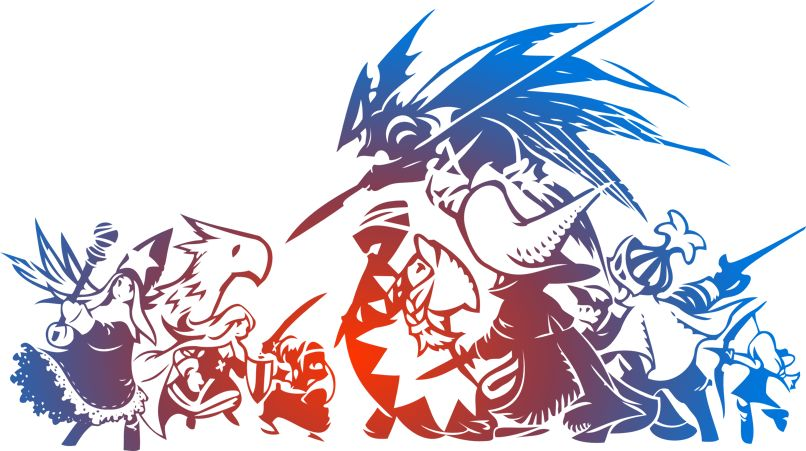
\includegraphics[width=\columnwidth]{./art/images/tactics.jpg}
%
%\\\\
%
\vfill
%
\ofboxwithtitle{Battlefield}{
The battlefield is divided into four rows: a front and a back row for each party.
At the start of a battle, every combatant decides for one of their side's two rows.
Whenever the front row of a party is empty, all combatants of that party are immediately pushed to their front row.
All actions have an effect has a \acc{Range} that indicates which rows it can target:\\
\acc{Self:} can only target yourself.\\
\acc{Close:} can target anyone in your own row.\\
\acc{Melee:} while in the front row, can target anyone in your party or the enemy front row.
Can also target enemies in their back row, but all damage dealt is halved. 
While in the back row, can only target your party.\\
\acc{Ranged:} while in the front row, can target any row. While in the back row, can target any row except the enemy back row.\\
\acc{Artillery:} can target anyone on the battlefield.
}
%
\vfill
%
\ofboxwithtitle{Example: Battlefield}
{
	Cecil and his friends fight the Magus Sisters with the current layout as shown below.
	It is Mindy's turn and she uses her Passado ability, which damages enemies in a 1u Front shape.
	She targets Cecil and Yang and afterwards ends her turn by selecting Sandy as next in order.
	Then it is Tella's turn and he uses the Ranged spell Fire and he targets Mindy with it, dealing enough damage to cause KO.
	Tella ends his turn by picking Cecil as next in order.
	Now it is Sandy's turn and she uses her Razzia ability which damages enemies in a Line shape and she targets Cid and Tella with it, causing KO to both of them.
	Then it is Cecil's turn and because the enemy Front Row is empty now, he can target the Back Row with Melee Attacks.
	He chooses to Attack Sandy and deals enough damage to KO her.
	Cindy, as the last standing Magus Sister, tries to Escape, but fails the evasion check.
	Finally, Yang takes his turn and uses the Melee Kick ability on Cindy and deals enough damage with it to cause her KO.
	The Magus Sisters are defeated!
}
%
\ofrow
%
\begin{figure}[h!]
	\centering
	\begin{tikzpicture}[]
	\tikzstyle{player}=[thick, fill=blue!15!white, draw, circle, align=center, minimum size = 0.125\columnwidth]					
	\tikzstyle{enemy}=[thick, fill=red!20!white, draw, circle, align=center, minimum size = 0.125\columnwidth]					
	
	\node[](txt)at (-0.375\columnwidth, 0.35\columnwidth) {\acc{Back}};
	\node[](txt)at (-0.125\columnwidth, 0.35\columnwidth) {\acc{Front}};
	\node[](txt)at (0.375\columnwidth, 0.35\columnwidth) {\accrf{Back}};
	\node[](txt)at (0.125\columnwidth, 0.35\columnwidth) {\accrf{Front}};
	
	\footnotesize
	\draw[color=accent, thick, dashed, -](-0.25\columnwidth, -0.3\columnwidth) -- (-0.25\columnwidth, 0.3\columnwidth);
	\draw[color=accent, thick, dashed, -](0, -0.3\columnwidth) -- (0, 0.3\columnwidth);
	\draw[color=accent, thick, dashed, -](0.25\columnwidth, -0.3\columnwidth) -- (0.25\columnwidth, 0.3\columnwidth);

	\node[player](cecil)at (-0.125\columnwidth, 0.225\columnwidth) {Cecil};
	\node[player](cid)at (-0.125\columnwidth, 0.075\columnwidth) {Cid};
	\node[player](tella)at (-0.375\columnwidth, -0.075\columnwidth) {Tella};
	\node[player](yang)at (-0.125\columnwidth, -0.225\columnwidth) {Yang};

	\node[enemy](sandy)at (0.375\columnwidth, 0.225\columnwidth) {Sandy};
	\node[enemy](cindy)at (0.125\columnwidth, 0.075\columnwidth) {Mindy};
	\node[enemy](mindy)at (0.375\columnwidth, -0.075\columnwidth) {Cindy};
	
	\end{tikzpicture}
\end{figure}
%
%\clearpage
